% Version: 1.1
% Description: 70GHz Clock Generation Architecture via Phase Interpolation - Landscape with Phase Noise Derivations
\documentclass[12pt]{article}
\usepackage{amsmath}
\usepackage{amssymb}
\usepackage{tikz}
\usepackage{pgfplots}
\pgfplotsset{compat=1.18}
\usetikzlibrary{shapes.geometric, arrows.meta, positioning, calc}
\usepackage[landscape, margin=0.2in]{geometry}

\begin{document}

\section*{System Architecture \& Phase Noise Transfer: 70GHz Clock Generation}

\subsection*{1. Top-Level Architecture}

\begin{center}
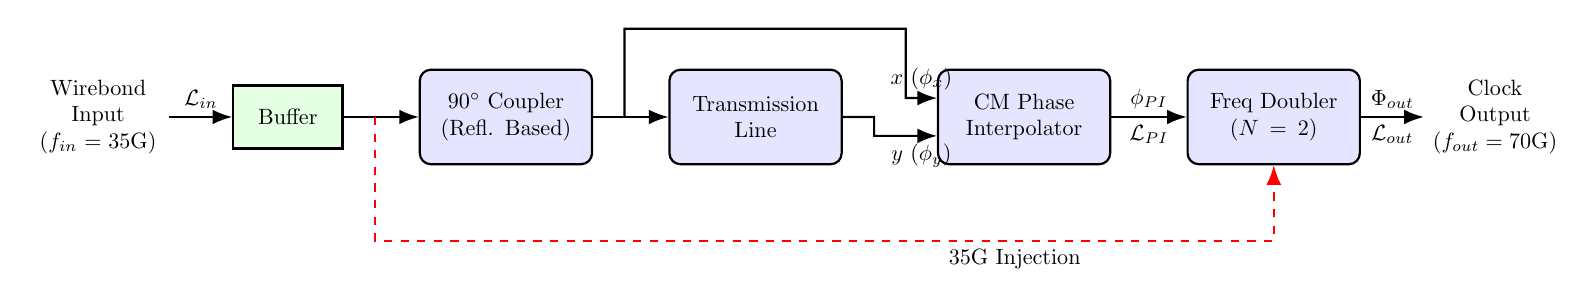
\begin{tikzpicture}[
    scale=0.8, transform shape,
    auto, thick,
    block/.style={rectangle, draw, fill=blue!10, text width=2.5cm, text centered, rounded corners, minimum height=1.5cm},
    smallblock/.style={rectangle, draw, fill=green!10, text width=1.5cm, text centered, minimum height=1cm},
    line/.style={draw, -{Latex[length=2.5mm]}}
]

    % Nodes
    \node (wirebond) [text width=2cm, text centered] {Wirebond Input \\ ($f_{in}=35\text{G}$)};
    \node (buffer) [smallblock, right=1cm of wirebond] {Buffer};

    % Series: Coupler -> TLine
    \node (coupler) [block, right=1.2cm of buffer] {90$^\circ$ Coupler \\ (Refl. Based)};
    \node (tline) [block, right=1.2cm of coupler] {Transmission Line};

    \node (cmpi) [block, right=1.5cm of tline] {CM Phase Interpolator};
    \node (doubler) [block, right=1.2cm of cmpi] {Freq Doubler \\ ($N=2$)};
    \node (output) [text width=2cm, text centered, right=1cm of doubler] {Clock Output ($f_{out}=70\text{G}$)};

    % Input to Buffer
    \path [line] (wirebond) -- node[above] {$\mathcal{L}_{in}$} (buffer);

    % Buffer to Coupler (with split for injection path)
    \coordinate (split0) at ([xshift=0.5cm]buffer.east);
    \draw [line] (buffer.east) -- (split0) -- (coupler.west);

    % Coupler to T-Line (with tap 1 for CMPI x)
    \coordinate (split1) at ([xshift=0.5cm]coupler.east);
    \draw [line] (coupler.east) -- (split1) -- (tline.west);

    % Tap 1: Jumps over T-Line to CMPI x input
    \coordinate (high_y) at ([yshift=1.4cm]split1);
    \coordinate (mid_x) at ([xshift=-0.5cm, yshift=3mm]cmpi.west);
    \draw [line] (split1) -- (high_y) -| (mid_x) -- node[above] {$x$ ($\phi_x$)} ([yshift=3mm]cmpi.west);

    % Tap 2: After T-Line to CMPI y input
    \coordinate (tline_out) at ([xshift=0.5cm]tline.east);
    \coordinate (mid_y) at ([xshift=-0.5cm, yshift=-3mm]cmpi.west);
    \draw [line] (tline.east) -- (tline_out) |- (mid_y) -- node[below] {$y$ ($\phi_y$)} ([yshift=-3mm]cmpi.west);

    % PI to Doubler
    \path [line] (cmpi) -- node [above] {$\phi_{PI}$} node[below] {$\mathcal{L}_{PI}$} (doubler);

    % Doubler to Output
    \path [line] (doubler) -- node [above] {$\Phi_{out}$} node[below] {$\mathcal{L}_{out}$} (output);

    % Injection path (routed cleanly underneath everything)
    \coordinate (inj_path) at ([yshift=-1.2cm]tline.south);
    \draw [-{Latex[length=2.5mm]}, dashed, red, thick] (split0) |- (inj_path)
        -- node [below, text=black] {35G Injection}
        (inj_path -| doubler.south) -- (doubler.south);

\end{tikzpicture}
\end{center}

\vspace{1cm}
\subsection*{2. Theoretical Derivations: Jitter \& Phase Noise}

\textbf{Phase Noise Multiplication:} \\
For a generic frequency multiplier $N$, the relation between input and output phase noise is:
\begin{equation}
    \mathcal{L}_{out}(f_{off}) = \mathcal{L}_{in}(f_{off}) + 20\log_{10}(N) + \mathcal{L}_{add}(f_{off})
\end{equation}
Substituting $N=2$ for the doubler, the theoretical minimum degradation is:
\begin{equation}
    \mathcal{L}_{out}(f_{off}) \approx \mathcal{L}_{in}(f_{off}) + 6\text{ dB}
\end{equation}

\textbf{Absolute Jitter Preservation:} \\
Time jitter $\sigma_t$ relates to integrated phase variance $\sigma_\phi^2$ and carrier frequency $f_c$:
\begin{equation}
    \sigma_t = \frac{\sqrt{\sigma_\phi^2}}{2\pi f_c}
\end{equation}
When passing through the doubler, phase variance increases by a factor of $N^2$, but the frequency also scales by $N$:
\begin{equation}
    \sigma_{t,out} = \frac{\sqrt{N^2 \sigma_{\phi,in}^2}}{2\pi (N f_{in})} = \frac{N \sigma_{\phi,in}}{N (2\pi f_{in})} = \sigma_{t,in}
\end{equation}
Thus, ideal absolute jitter is preserved at 70 GHz.

\newpage
\subsection*{3. Phase Noise Profiles \& Injection Locking Dynamics}

\begin{center}
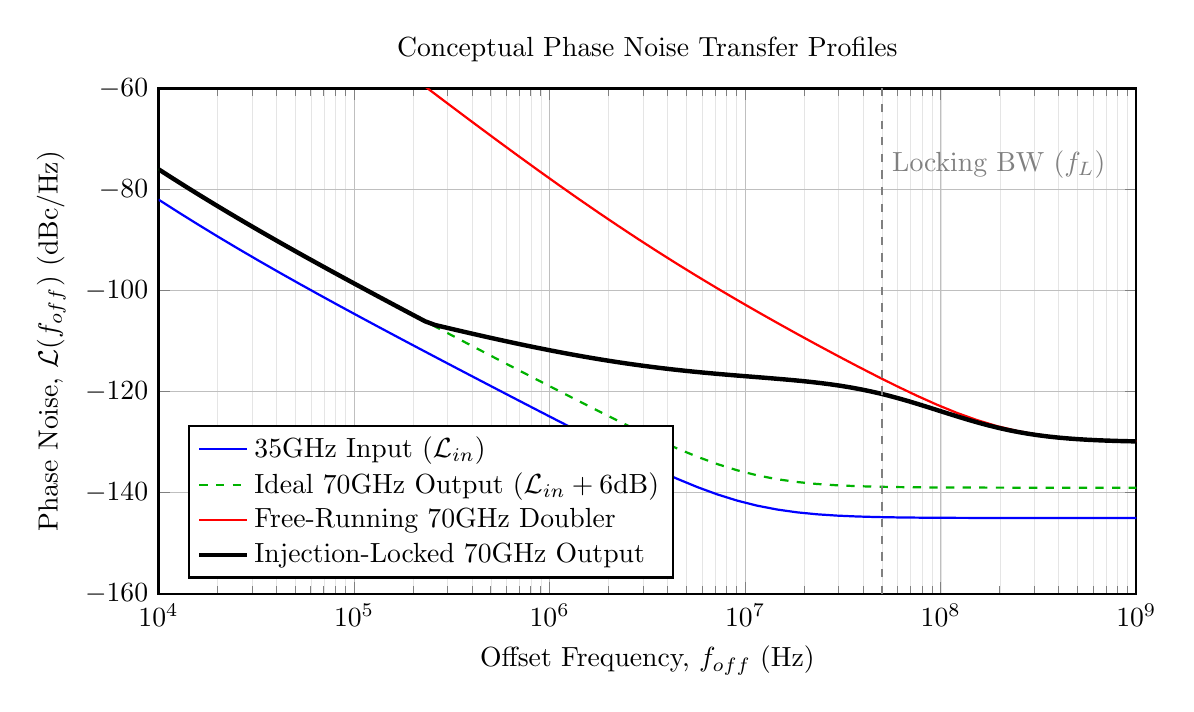
\begin{tikzpicture}

\begin{axis}[
    width=14cm,
    height=8cm,
    xmode=log,
    xmin=1e4, xmax=1e9,
    ymin=-160, ymax=-60,
    grid=both,
    grid style={line width=.1pt, draw=gray!20},
    major grid style={line width=.2pt,draw=gray!50},
    xlabel={Offset Frequency, $f_{off}$ (Hz)},
    ylabel={Phase Noise, $\mathcal{L}(f_{off})$ (dBc/Hz)},
    title={Conceptual Phase Noise Transfer Profiles},
    legend pos=south west,
    legend cell align={left},
    thick
]

% 1. Input 35G Signal
\addplot[blue, domain=1e4:1e9, samples=50] 
    {-145 + 10*log10(1 + (1e6/x)^3 + (1e7/x)^2)};
\addlegendentry{35GHz Input ($\mathcal{L}_{in}$)}

% 2. Ideal Doubled Signal (Input + 6dB)
\addplot[green!70!black, dashed, domain=1e4:1e9, samples=50] 
    {-139 + 10*log10(1 + (1e6/x)^3 + (1e7/x)^2)};
\addlegendentry{Ideal 70GHz Output ($\mathcal{L}_{in} + 6\text{dB}$)}

% 3. Free-running Doubler (acts like a noisy VCO)
\addplot[red, domain=1e4:1e9, samples=50] 
    {-130 + 10*log10(1 + (5e7/x)^3 + (2e8/x)^2)};
\addlegendentry{Free-Running 70GHz Doubler}

% 4. Injection Locked Output
% Tracks the ideal +6dB curve until the locking bandwidth (e.g., 50MHz), then follows free-running
\addplot[black, ultra thick, domain=1e4:1e9, samples=100] 
    {max(
        -139 + 10*log10(1 + (1e6/x)^3 + (1e7/x)^2), 
        -130 + 10*log10(1 + (5e7/x)^3 + (2e8/x)^2) - 10*log10(1 + (5e7/x)^2)
    )};
\addlegendentry{Injection-Locked 70GHz Output}

% Locking Bandwidth Marker
\draw[dashed, thick, gray] (axis cs:5e7,-160) -- (axis cs:5e7,-60) node[pos=0.85, right] {Locking BW ($f_L$)};

\end{axis}
\end{tikzpicture}
\end{center}

\subsection*{4. Phase Interpolation Phasor Diagram (Revised)}

\begin{center}
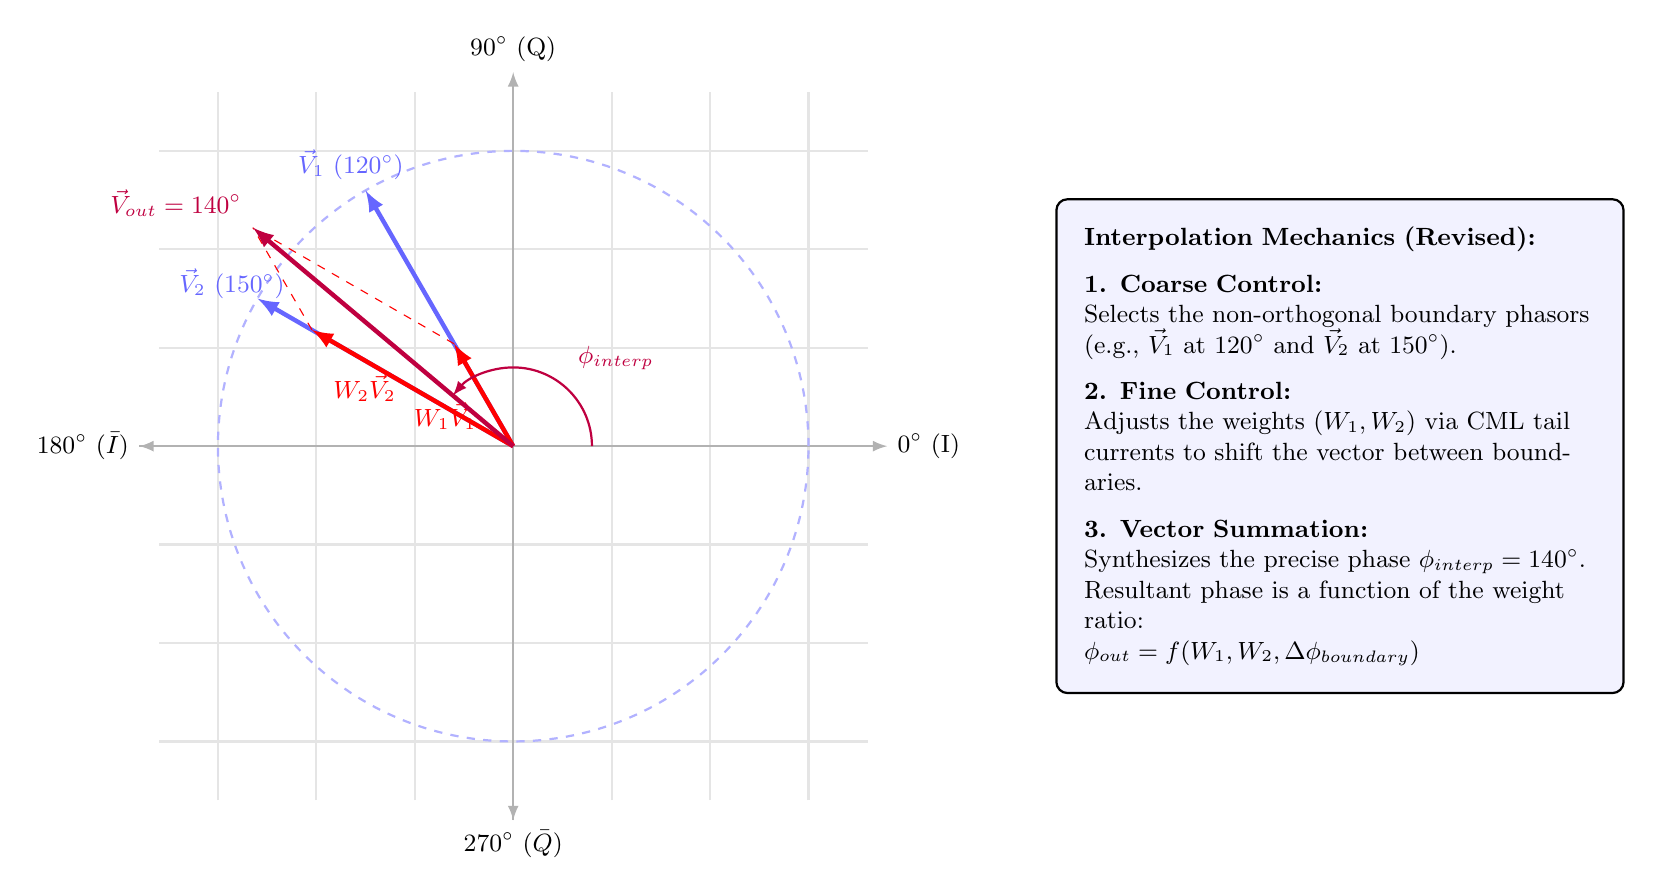
\begin{tikzpicture}[
    >=latex,
    scale=2.5,
    thick,
    font=\small
]

    % Grid and axes
    \draw[gray!20, step=0.5] (-1.8,-1.8) grid (1.8,1.8);
    \draw[->, gray!60] (-1.9,0) -- (1.9,0) node[right, black] {$0^\circ$ (I)};
    \draw[->, gray!60] (0,-1.9) -- (0,1.9) node[above, black] {$90^\circ$ (Q)};
    \draw[->, gray!60] (0,0) -- (-1.9,0) node[left, black] {$180^\circ$ ($\bar{I}$)};
    \draw[->, gray!60] (0,0) -- (0,-1.9) node[below, black] {$270^\circ$ ($\bar{Q}$)};

    % Unit circle
    \draw[dashed, blue!30] (0,0) circle (1.5);

    % Define Angles
    \def\angA{120}
    \def\angB{150}
    \def\angOut{140}
    \def\R{1.5}

    % Coarse Boundary Vectors (V1 and V2)
    \draw[->, ultra thick, blue!60] (0,0) -- (\angA:\R) node[pos=1.1] {$\vec{V}_1$ (120$^\circ$)};
    \draw[->, ultra thick, blue!60] (0,0) -- (\angB:\R) node[pos=1.1] {$\vec{V}_2$ (150$^\circ$)};

    % Calculation for W1 and W2 to get exactly 140 degrees
    % Using law of sines in the vector triangle:
    % W2/sin(140-120) = W1/sin(150-140)
    % W2/sin(20) = W1/sin(10) => W2 = W1 * (sin(20)/sin(10))
    \def\Wone{0.6}
    \def\Wtwo{1.18} % Approx W1 * sin(20)/sin(10) for 140 deg

    % Weighted Component Vectors (Red)
    \draw[->, ultra thick, red] (0,0) -- (\angA:\Wone) node[midway, below left=-2pt] {$W_1 \vec{V}_1$};
    \draw[->, ultra thick, red] (0,0) -- (\angB:\Wtwo) node[midway, left=2pt] {$W_2 \vec{V}_2$};

    % Parallelogram construction
    \coordinate (V1w) at (\angA:\Wone);
    \coordinate (V2w) at (\angB:\Wtwo);
    \coordinate (Vout) at ($(V1w)+(V2w)$);
    
    \draw[dashed, red, thin] (V1w) -- (Vout);
    \draw[dashed, red, thin] (V2w) -- (Vout);

    % Resultant Interpolated Vector
    \draw[->, ultra thick, purple] (0,0) -- (Vout) node[above left] {$\vec{V}_{out} = 140^\circ$};

    % Phase Angle Arc
    \draw[->, thick, purple] (0.4,0) arc (0:\angOut:0.4) node[midway, right=10pt, yshift=5pt] {$\phi_{interp}$};

    % Legend/Explanation Box - Positioned to the right to avoid overlap
    \node[align=left, draw, fill=blue!5, rounded corners, inner sep=10pt, text width=6.5cm] at (4.2, 0) {
        \textbf{Interpolation Mechanics (Revised):} \\[1.5ex]
        \textbf{1. Coarse Control:} \\
        Selects the non-orthogonal boundary phasors \\
        (e.g., $\vec{V}_1$ at $120^\circ$ and $\vec{V}_2$ at $150^\circ$). \\[1.5ex]
        \textbf{2. Fine Control:} \\
        Adjusts the weights ($W_1, W_2$) via CML tail \\
        currents to shift the vector between boundaries. \\[1.5ex]
        \textbf{3. Vector Summation:} \\
        Synthesizes the precise phase $\phi_{interp} = 140^\circ$. \\
        Resultant phase is a function of the weight ratio: \\
        $\phi_{out} = f(W_1, W_2, \Delta\phi_{boundary})$
    };

\end{tikzpicture}
\end{center}

\subsection*{5. Bode Plot}

\begin{center}
    
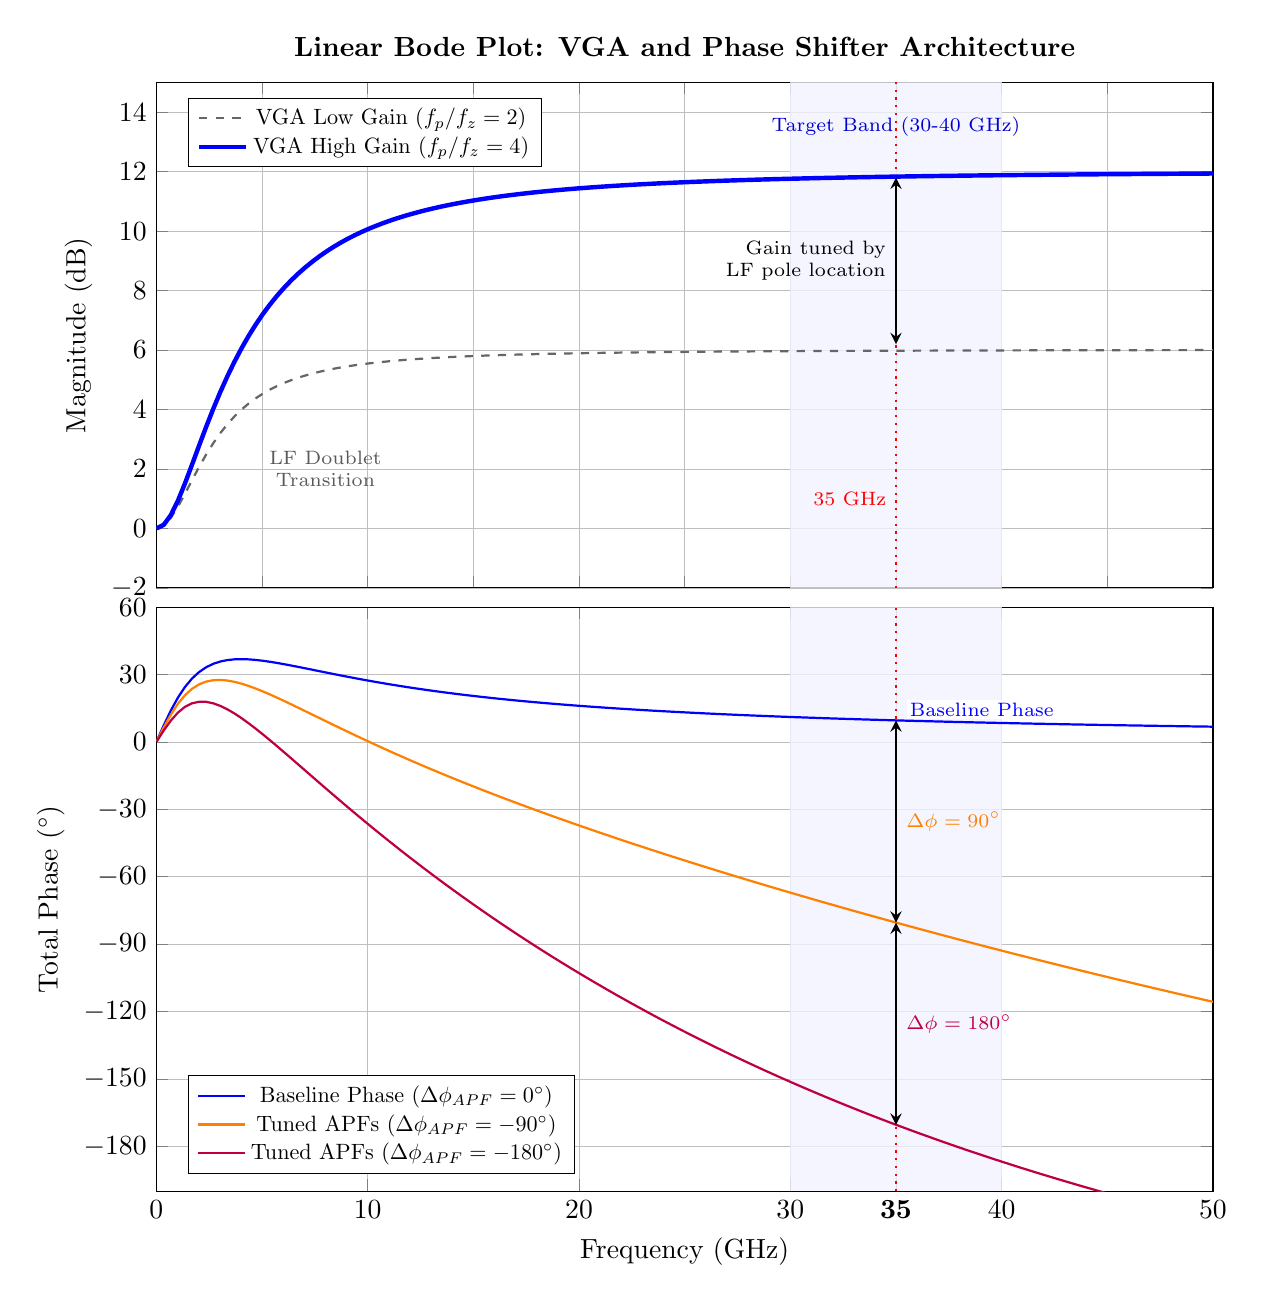
\begin{tikzpicture}

    % --- MAGNITUDE PLOT ---
    \begin{axis}[
        name=mag,
        width=15cm,
        height=8cm,
        xmode=normal, % Linear scale
        xmin=0, xmax=50,
        ymin=-2, ymax=15,
        grid=both,
        grid style={line width=.1pt, draw=gray!20},
        major grid style={line width=.2pt, draw=gray!50},
        ylabel={Magnitude (dB)},
        xticklabel=\empty, 
        title={\textbf{Linear Bode Plot: VGA and Phase Shifter Architecture}},
        legend pos=north west,
        legend style={nodes={scale=0.8, transform shape}}
    ]

        % Highlighted 30-40 GHz Region
        \fill[blue!5, opacity=0.8] (axis cs:30,-2) rectangle (axis cs:40,15);
        \node[text=blue!80!black, font=\scriptsize] at (axis cs:35, 13.5) {Target Band (30-40 GHz)};

        % Dotted Line at 35 GHz
        \draw[dotted, thick, red] (axis cs:35,-2) -- (axis cs:35,15);
        \node[text=red, font=\scriptsize, anchor=east] at (axis cs:35, 1) {35 GHz};

        % VGA Low Gain State: fz = 2 GHz, fp = 4 GHz -> ~6dB HF gain
        \addplot[dashed, gray!80!black, thick, domain=0.01:50, samples=150] 
            {10*log10( (1 + (x/2)^2) / (1 + (x/4)^2) )};
        \addlegendentry{VGA Low Gain ($f_p/f_z = 2$)}

        % VGA High Gain State: fz = 2 GHz, fp = 8 GHz -> ~12dB HF gain
        \addplot[blue, ultra thick, domain=0.01:50, samples=150] 
            {10*log10( (1 + (x/2)^2) / (1 + (x/8)^2) )};
        \addlegendentry{VGA High Gain ($f_p/f_z = 4$)}

        % Annotations for Magnitude
        \draw[<->, >=stealth, thick] (axis cs:35, 6.2) -- (axis cs:35, 11.8) 
            node[midway, left, font=\scriptsize, align=right] {Gain tuned by\\LF pole location};
            
        \node[font=\scriptsize, align=center, text=gray!70!black] at (axis cs:8, 2) {LF Doublet\\Transition};

    \end{axis}

    % --- PHASE PLOT ---
    \begin{axis}[
        name=phase,
        at={(mag.below south west)},
        anchor=north west,
        width=15cm,
        height=9cm,
        xmode=normal, % Linear scale
        xmin=0, xmax=50,
        ymin=-200, ymax=60,
        grid=both,
        grid style={line width=.1pt, draw=gray!20},
        major grid style={line width=.2pt, draw=gray!50},
        xlabel={Frequency (GHz)},
        ylabel={Total Phase ($^\circ$)},
        xtick={0, 10, 20, 30, 35, 40, 50},
        xticklabels={0, 10, 20, 30, \textbf{35}, 40, 50},
        ytick={60, 30, 0, -30, -60, -90, -120, -150, -180},
        legend pos=south west,
        legend style={nodes={scale=0.8, transform shape}}
    ]

        % Highlighted 30-40 GHz Region
        \fill[blue!5, opacity=0.8] (axis cs:30,-200) rectangle (axis cs:40,60);

        % Dotted Line at 35 GHz
        \draw[dotted, thick, red] (axis cs:35,-200) -- (axis cs:35,60);

        % Baseline Phase (VGA High Gain only, APF f0 = infinity)
        \addplot[blue, thick, domain=0.01:50, samples=150] 
            {atan(x/2) - atan(x/8)};
        \addlegendentry{Baseline Phase ($\Delta\phi_{APF} = 0^\circ$)}

        % Tuned Phase 1: APF f0 = 84.5 GHz -> -90 deg shift at 35GHz
        \addplot[orange, thick, domain=0.01:50, samples=150] 
            {atan(x/2) - atan(x/8) - 4*atan(x/84.5)};
        \addlegendentry{Tuned APFs ($\Delta\phi_{APF} = -90^\circ$)}

        % Tuned Phase 2: APF f0 = 35 GHz -> -180 deg shift at 35GHz
        \addplot[purple, thick, domain=0.01:50, samples=150] 
            {atan(x/2) - atan(x/8) - 4*atan(x/35)};
        \addlegendentry{Tuned APFs ($\Delta\phi_{APF} = -180^\circ$)}
            
        % Annotations for Phase Shifts at 35 GHz
        % Baseline phase at 35GHz is approx +9.6 degrees due to residual LF doublet phase
        \draw[<->, >=stealth, thick] (axis cs:35, 9.6) -- (axis cs:35, -80.4) 
            node[midway, right, font=\scriptsize, text=orange] {$\Delta\phi = 90^\circ$};
            
        \draw[<->, >=stealth, thick] (axis cs:35, -80.4) -- (axis cs:35, -170.4) 
            node[midway, right, font=\scriptsize, text=purple] {$\Delta\phi = 180^\circ$};

        \node[anchor=south west, font=\scriptsize, text=blue, fill=white, inner sep=1pt] at (axis cs:35.5, 10) {Baseline Phase};
        
    \end{axis}

\end{tikzpicture}
\end{center}

\end{document}
